\chapter{Light as an Eigenvalue Problem}
\label{ch:light-eigenvalue}

\begin{chapterlead}
What does it mean to say that light has ``modes''? Every physicist who has
worked with optical cavities, waveguides, or photonic crystals eventually
invokes a set of modes---discrete field patterns, each oscillating at a
single frequency. This chapter shows where those modes come from:
they are eigenvalues and eigenvectors of an operator built from
Maxwell's equations and the material response of the medium.
The structure of that operator---whether it is self-adjoint or not---controls
everything that follows in this book. We shall derive the eigenvalue
problem carefully, explain why it takes the form it does, explore its
mathematical structure through a variational principle, and illustrate it
with a worked one-dimensional example before giving a preview of what
happens when the operator loses its self-adjoint character.Ha hahahahahaahahahah.aaaaaaaaaaaaaabbbbbbbbbbbbbbbbbbbb
\end{chapterlead}


%% ================================================================
\section{Maxwell's equations in matter}
\label{sec:maxwell-matter}

We begin with the macroscopic Maxwell equations in a linear, time-invariant
medium with no free charges or currents:
\begin{align}
 Hahahahahahah.aaaaaaaaaaaaaaaabbbbbbbbbbbbbbbbbbbbbb \curl \EE(\rr,t) &= -\pdv{\BB(\rr,t)}{t}, \label{eq:faraday}\\[4pt]
 \curl \HH(\rr,t) &= \phantom{-}\pdv{\DD(\rr,t)}{t}, \label{eq:ampere}\\[4pt]
 \divg \DD(\rr,t) &= 0, \label{eq:gauss-e}\\[4pt]
 \divg \BB(\rr,t) &= 0. \label{eq:gauss-m}
\end{align}
These four equations, supplemented by constitutive relations connecting
$\DD$ to $\EE$ and $\BB$ to $\HH$, form the complete classical description of
electromagnetic fields in matter. Nothing in this book requires quantum
electrodynamics; the entire non-Hermitian structure we shall develop is
already present at the level of classical Maxwell theory.

In the simplest case the constitutive relations are local and instantaneous:
\begin{equation}
 \DD(\rr,t) = \epsvac\,\epsr(\rr)\,\EE(\rr,t),
 \qquad
 \BB(\rr,t) = \muvac\,\mur(\rr)\,\HH(\rr,t).
 \label{eq:constitutive-simple}
\end{equation}
Here $\epsr(\rr)$ and $\mur(\rr)$ are the relative permittivity and
permeability, which we allow to vary in space but, for now, take to be real
and positive. These assumptions will be progressively relaxed in later
chapters: Chapter~\ref{ch:loss-gain-dispersion} introduces complex and
frequency-dependent $\epsr$, Chapter~\ref{ch:qnm} opens the system to
radiation, and Chapter~\ref{ch:pt-symmetric} considers the special spatial
symmetry of balanced gain and loss.

The constitutive relations~\eqref{eq:constitutive-simple} encode all material
information available to the Maxwell operator. From the standpoint of
the eigenvalue problem we are about to derive, $\epsr(\rr)$ is the central
material input: it controls the spatial pattern of the eigenmodes, the
distribution of eigenfrequencies, and---when it becomes complex---the transition
from Hermitian to non-Hermitian spectral theory.

\begin{booknote}[Why macroscopic Maxwell?]
A monograph on non-Hermitian photonics could, in principle, start from the
microscopic Maxwell equations and derive macroscopic constitutive relations.
We choose to start at the macroscopic level for two reasons. First, the
non-Hermitian phenomena we study---complex eigenfrequencies, exceptional
points, non-reciprocal skin effects---arise already in the macroscopic theory
and do not require a microscopic derivation to be well posed. Second, the
macroscopic framework is what connects directly to photonic-crystal band
computations, scattering-matrix measurements, and device design.
\end{booknote}

\begin{figure}[t]
 \centering
 
\includegraphics[width=0.98\textwidth]{fig_f1_maxwell_operator_map.pdf}
 \caption{Haahahahahahah.aaaaaaaaaaaaaaaaaabbbbbbbbbbbbbbbbbbb The Maxwell-first route followed in this book. Starting from macroscopic Maxwell equations and constitutive relations, eliminating one field gives the curl--curl operator. When the material is real, the surface term vanishes, and the transverse field space is complete, the operator gives Hermitian photonics. Loss or gain, radiation boundaries, dispersion, and projection onto a subspace lead to the non-Hermitian structures studied in later chapters.}
 \label{fig:maxwell-operator-map}
\end{figure}


%% ================================================================
\section{The frequency-domain eigenproblem hahahahahaaaaaaaaaaaaaabbbbbbbbbbbbbbbbbbbbbb}
\label{sec:freq-domain}

\subsection{Harmonic fields and the time-frequency correspondence}
\label{ssec:harmonic}

For a time-invariant medium it is natural to look for solutions with
harmonic time dependence. We write
\begin{equation}
 \EE(\rr,t) = \Re\!\bigl[\EE(\rr)\,e^{-i\omega t}\bigr],
 \qquad
 \HH(\rr,t) = \Re\!\bigl[\HH(\rr)\,e^{-i\omega t}\bigr],
 \label{eq:harmonic-ansatz}
\end{equation}
where $\omega$ is a real angular frequency and $\EE(\rr)$, $\HH(\rr)$ are
complex-valued spatial amplitudes. At this stage $\omega$ may be regarded
as the real frequency of a harmonic drive. Later, when we solve source-free
open or lossy eigenvalue problems, the same convention will allow
$\omega$ itself to become complex. The sign convention $e^{-i\omega t}$
is standard in the optics and photonics literature; the condensed-matter
convention $e^{+i\omega t}$ leads to conjugated constitutive parameters but
no change in the physics.

The physical content of the harmonic ansatz is that once we know the spatial
amplitude $\EE(\rr)$ at a single frequency $\omega$, we know the complete
space-time field at that frequency. The general time-domain solution is then
recovered by Fourier superposition. The advantage of the frequency-domain
formulation is that the partial differential equations in space-time reduce
to ordinary or partial differential equations in space alone---eigenvalue
problems whose solutions organize the entire electromagnetic response.

\subsection{Deriving the curl--curl eigenproblem}
\label{ssec:curlcurl-derive}

Substituting \eqref{eq:harmonic-ansatz} into Faraday's law
\eqref{eq:faraday} and Amp\`ere's law \eqref{eq:ampere} gives
\begin{align}
 \curl \EE &= i\omega\,\muvac\mur\,\HH, \label{eq:faraday-freq}\\[3pt]
 \curl \HH &= -i\omega\,\epsvac\epsr\,\EE. \label{eq:ampere-freq}
\end{align}
These are two coupled first-order equations for $\EE$ and $\HH$. We can
decouple them by eliminating one field. Applying $\curl$ to
\eqref{eq:ampere-freq} and inserting \eqref{eq:faraday-freq}, we obtain
the \emph{curl--curl eigenproblem for the electric field}:
\begin{equation}
 \boxed{
 \curl\!\left[\frac{1}{\mur(\rr)}\,\curl\EE(\rr)\right]
 = \frac{\omega^2}{c^2}\,\epsr(\rr)\,\EE(\rr).
 }
 \label{eq:curlcurl-E}
\end{equation}
Here $c = 1/\sqrt{\epsvac\muvac}$ is the speed of light in vacuum.
Equation~\eqref{eq:curlcurl-E} is a generalized eigenvalue problem:
the operator on the left acts on $\EE$, the eigenvalue is
$\omega^2/c^2$, and the ``weight'' on the right is the
position-dependent $\epsr(\rr)$.

The elimination procedure is worth understanding in detail, because it
reveals where the operator structure comes from. Writing the two steps
explicitly:
\begin{enumerate}
 \item Use Faraday's law to express the magnetic field as
 $\HH=(i\omega\muvac\mur)^{-1}\curl\EE$.
 \item Insert this expression into Amp\`ere's law:
 \[
 \curl\!\left[\frac{1}{i\omega\muvac\mur}\curl\EE\right]
 = -i\omega\epsvac\epsr\EE,
 \]
 and multiply by $i\omega\muvac$ to obtain
 $\curl[(1/\mur)\curl\EE]=(\omega^2/c^2)\epsr\EE$.
\end{enumerate}
The curl--curl structure on the left is the price we pay for eliminating
one field; the $\epsr$ weight on the right arises from the constitutive
relation. Together they produce a second-order operator in space---directly
analogous to the kinetic-energy operator $-\nabla^2$ in quantum mechanics,
but with the curl replacing the gradient and the permittivity entering as
a generalized eigenvalue weight rather than as an additive potential.

\subsection{The magnetic-field formulation}
\label{ssec:h-formulation}

An analogous equation can be written for $\HH$ alone. Eliminating $\EE$
from \eqref{eq:faraday-freq}--\eqref{eq:ampere-freq} yields
\begin{equation}
 \curl\!\left[\frac{1}{\epsr(\rr)}\,\curl\HH(\rr)\right]
 = \frac{\omega^2}{c^2}\,\mur(\rr)\,\HH(\rr).
 \label{eq:curlcurl-H}
\end{equation}
For non-magnetic media ($\mur = 1$ everywhere), \eqref{eq:curlcurl-H}
simplifies to the standard form used in photonic-crystal theory:
\begin{equation}
 \Mop\,\HH(\rr)
 \;\equiv\;
 \curl\!\left[\frac{1}{\epsr(\rr)}\,\curl\HH(\rr)\right]
 = \frac{\omega^2}{c^2}\,\HH(\rr).
 \label{eq:maxwell-op-H}
\end{equation}
The operator $\Mop$ defined here will be a central object throughout
this book~\cite{figotin2004hamiltonian,raman2010photonic}. Its properties---self-adjointness, compactness of the resolvent,
spectral structure---depend critically on three ingredients:
\begin{enumerate}
 \item the spatial profile of $\epsr(\rr)$ (real or complex, bounded or
 unbounded, periodic or not);
 \item the boundary conditions imposed on $\HH$ at the edges of the
 computational or physical domain;
 \item the function space on which $\Mop$ acts.
\end{enumerate}

Both the $\EE$-field and $\HH$-field formulations are exact restatements
of Maxwell's equations for harmonic fields. However, the $\HH$-field form
has a practical advantage for non-magnetic media: the eigenvalue
$\omega^2/c^2$ appears with a trivial (unit) weight on the right, making
the operator $\Mop$ a standard eigenvalue problem rather than a generalized
one. For this reason, most photonic band-structure codes work with the
$\HH$ formulation, and we shall use $\Mop$ as the default Maxwell operator
throughout this book unless otherwise stated.

\subsection{The divergence constraint}
\label{ssec:divergence}

The curl--curl operator has a large null space: any gradient field
$\HH = \nabla\phi$ satisfies $\curl\HH = 0$ and therefore
$\Mop(\nabla\phi) = 0$. These spurious zero-frequency solutions are
not physical propagating modes; in general they do not satisfy the
transverse constraint $\divg\BB = \muvac\divg\HH = 0$ (or equivalently
$\divg(\epsr\EE) = 0$ in the $\EE$ formulation), and even when a harmonic
gradient field survives as a static zero mode it must be separated from
the dynamical spectrum.

In analytical work, the divergence condition is enforced by restricting
the domain of $\Mop$ to transverse (divergence-free) fields:
\begin{equation}
 \mathcal{H}_{\mathrm{div}} = \bigl\{
 \HH \in L^2(\Omega;\mathbb{C}^3) \;\big|\;
 \divg\HH = 0,\;\text{plus boundary conditions}
 \bigr\}.
 \label{eq:div-free-space}
\end{equation}
On this restricted domain, the null space is eliminated and $\Mop$ becomes
positive semi-definite: all non-static eigenvalues satisfy
$\omega^2/c^2 \ge 0$. This is physically obvious---squared frequencies
cannot be negative in a closed, lossless medium---but mathematically it
relies on the restriction to divergence-free fields and on the treatment
of possible harmonic zero modes.

In numerical work (Chapter~\ref{ch:numerics}), the divergence constraint
must be enforced explicitly, either through a penalty term, a Lagrange
multiplier, or a compatible discretization, such as N\'ed\'elec edge
elements combined with a proper treatment of the gradient null space.
Failure to control this constraint produces spurious modes near
$\omega = 0$ that can contaminate the physical spectrum.


%% ================================================================
\section{Self-adjointness and its physical meaning}
\label{sec:self-adjoint}

\subsection{The electromagnetic inner product}
\label{ssec:em-inner-product}

To ask whether $\Mop$ is self-adjoint, we need an inner product. For
two vector fields $\mathbf{F}$ and $\mathbf{G}$ defined over a domain
$\Omega$, the natural electromagnetic inner product is
\begin{equation}
 \langle \mathbf{F},\,\mathbf{G}\rangle
 \;=\;
 \int_\Omega \mathbf{F}^*(\rr)\cdot\mathbf{G}(\rr)\;\dd^3 r.
 \label{eq:inner-product-plain}
\end{equation}
We also define a weighted inner product:
\begin{equation}
 \langle \mathbf{F},\,\mathbf{G}\rangle_{\eps}
 \;=\;
 \int_\Omega \mathbf{F}^*(\rr)\cdot\epsr(\rr)\,\mathbf{G}(\rr)\;\dd^3 r.
 \label{eq:inner-product}
\end{equation}
Chapter~\ref{ch:energy-inner} develops the physical interpretation of these
inner products in terms of electromagnetic energy.

\subsection{Integration by parts and the boundary term}
\label{ssec:ibp}

We now ask: under what conditions does $\Mop$ satisfy
$\langle\mathbf{F},\,\Mop\mathbf{G}\rangle
 = \langle\Mop\mathbf{F},\,\mathbf{G}\rangle$
for all admissible $\mathbf{F}$ and $\mathbf{G}$? The answer comes
from integration by parts. Using the vector identity
\begin{equation}
 \int_\Omega \mathbf{F}^*\cdot\bigl(\curl\mathbf{A}\bigr)\;\dd^3 r
 =
 \int_\Omega \bigl(\curl\mathbf{F}^*\bigr)\cdot\mathbf{A}\;\dd^3 r
 +
 \oint_{\partial\Omega}
 \bigl(\mathbf{F}^*\times\mathbf{A}\bigr)\cdot\nn\;\dd S,
 \label{eq:curl-ibp}
\end{equation}
applied twice with $\mathbf{A} = (1/\epsr)\curl\mathbf{G}$, one finds
that for $\mur = 1$ the bulk integrals are
symmetric provided $\epsr(\rr)$ is \emph{real}---so that the weight in
\eqref{eq:inner-product} commutes with complex conjugation---and the
surface integral
\begin{equation}
 \oint_{\partial\Omega}
 \left[
 \mathbf{F}^*\times\frac{1}{\epsr}\curl\mathbf{G}
+
 \left(\frac{1}{\epsr}\curl\mathbf{F}\right)^{\!*}\times\mathbf{G}
 \right]\cdot\nn\;\dd S
 = 0
 \label{eq:surface-vanish}
\end{equation}
vanishes. For a closed cavity with perfectly conducting walls
($\nn\times\EE = 0$ on $\partial\Omega$), this surface term is zero. For
a periodic medium with Bloch boundary conditions, it cancels between
opposite faces of the unit cell.

\subsection{The three conditions for Hermitian photonics}
\label{ssec:three-conditions}

\begin{takeaway}[Three conditions for Hermitian photonics]
The Maxwell curl--curl operator $\Mop$ is self-adjoint with respect to
$\langle\cdot,\cdot\rangle$ on divergence-free fields when three conditions
hold simultaneously:
(i)~$\epsr(\rr)$ is real and positive everywhere in $\Omega$
(or, more generally, Hermitian positive definite for anisotropic media);
(ii)~the boundary conditions on $\partial\Omega$ make the surface term
\eqref{eq:surface-vanish} vanish;
(iii)~the domain of $\Mop$ is a complete Hilbert space of transverse
fields, with static null modes removed or treated separately.
Remove any one of these and the spectral theory must be rebuilt.
\end{takeaway}

This result is the foundation on which the entire book rests. Each of the
physical mechanisms that produce non-Hermiticity in photonics can be traced
back to the violation of one of these three conditions:
\begin{itemize}
 \item \textbf{Material loss or gain} (Chapters~\ref{ch:loss-gain-dispersion}
 and~\ref{ch:pt-symmetric}): the permittivity acquires an imaginary part,
 $\epsr \to \epsr' + i\epsr''$, so the weight in
 \eqref{eq:inner-product} is no longer real~\cite{longhi2018parity}. The operator $\Mop$ is
 no longer formally self-adjoint, and its eigenvalues migrate off the
 real axis into the complex plane.
 \item \textbf{Radiation and openness} (Chapters~\ref{ch:boundaries}
 and~\ref{ch:qnm}): outgoing-wave boundary conditions (Sommerfeld
 radiation condition or perfectly matched layers) do not make the surface
 term vanish; instead, energy escapes through $\partial\Omega$. The
 resulting quasinormal modes have complex eigenfrequencies even when
 $\epsr$ is real~\cite{kristensen2011effective,vial2014quasimodal}.
 \item \textbf{Frequency dispersion}
 (Chapter~\ref{ch:loss-gain-dispersion}): when $\epsr$ depends on
 $\omega$, the eigenvalue problem~\eqref{eq:maxwell-op-H} becomes
 nonlinear in the eigenvalue, and the standard spectral theory of
 self-adjoint operators no longer applies directly~\cite{figotin2004hamiltonian}.
 \item \textbf{Projection onto a subspace}
 (Chapter~\ref{ch:maxwell-coupled-modes}): even when the full Maxwell
 operator is self-adjoint, projecting onto a few resonant modes produces
 an effective finite-dimensional Hamiltonian that is generically
 non-Hermitian, because the discarded modes act as an environment~\cite{alpeggiani2017quasinormal}.
\end{itemize}

These four roads to non-Hermiticity are not independent---many real systems
exhibit several simultaneously---but they provide a useful organizational
framework. A $\PT$-symmetric photonic crystal, for example, has
complex $\epsr$ (road~1), may be open to radiation (road~2), may involve
dispersive gain media (road~3), and is often modeled by a few-mode
effective Hamiltonian (road~4).


%% ================================================================
\section{The variational principle}
\label{sec:variational}

Self-adjoint operators with discrete spectra admit a powerful variational
characterization of their eigenvalues. For $\Mop$ on the space of
transverse fields in a closed domain, the Rayleigh quotient is
\begin{equation}
 R[\HH] = \frac{\displaystyle\int_\Omega
 \frac{1}{\epsr(\rr)}\,|\curl\HH(\rr)|^2\;\dd^3 r}
 {\displaystyle\int_\Omega |\HH(\rr)|^2\;\dd^3 r}
 = \frac{\langle\Mop\HH,\,\HH\rangle}{\langle\HH,\,\HH\rangle},
 \label{eq:rayleigh}
\end{equation}
and the fundamental eigenfrequency satisfies the min--max principle:
\begin{equation}
\frac{\omega_1^2}{c^2} = \min_{\HH \in \mathcal{H}_{\mathrm{div}}}
R[\HH].
 \label{eq:minmax}
\end{equation}
where the minimization is over nonzero fields in the dynamical transverse
subspace. Higher eigenfrequencies are obtained by successive minimization
over subspaces orthogonal to the previously found eigenmodes.

The variational principle gives immediate physical insight:
\begin{itemize}
 \item The lowest mode concentrates its magnetic field where
 $1/\epsr$ is smallest, i.e., where the permittivity is largest.
 This is the electromagnetic analogue of a quantum particle
 localizing in a potential well.
 \item Increasing $\epsr$ anywhere in $\Omega$ decreases all
 eigenfrequencies---intuitively, denser media slow light and lower the
 resonant frequencies.
 \item A band gap forms when no trial field can simultaneously satisfy
 the curl constraint and have low energy in a frequency window.
\end{itemize}

The variational principle also explains why the Hermitian eigenfrequencies
are always real: the Rayleigh quotient~\eqref{eq:rayleigh} is manifestly
real when $\epsr$ is real and positive, so $\omega_1^2/c^2$ is real and
non-negative, and $\omega_1$ is real.

\paragraph{What breaks when $\epsr$ is complex.}
If $\epsr$ has an imaginary part, the Rayleigh quotient becomes complex,
and the variational characterization fails: there is no longer a minimum
of a real functional, so the eigenfrequencies are not constrained to the
real axis. This is the variational way of seeing why complex $\epsr$
produces non-Hermitian photonics.


%% ================================================================
\section{Two-dimensional reductions}
\label{sec:2d-reductions}

Many photonic systems---photonic-crystal slabs, ridge waveguides, fiber
cross-sections---have a geometry that is invariant along one spatial
direction. For a system uniform along $z$, all fields can be decomposed
into components with a fixed $z$-dependence $e^{ik_z z}$. At $k_z = 0$
the vector Maxwell equations split into two independent scalar problems,
conventionally called \emph{transverse electric} (TE) and
\emph{transverse magnetic} (TM) polarizations. The common
two-dimensional photonic-crystal convention: TM denotes the scalar
$E_z$ problem and TE denotes the scalar $H_z$ problem. Some waveguide
texts use the opposite language relative to the propagation direction, so
the field component should always be checked.

\subsection{TM polarization}
\label{ssec:tm}

In TM polarization the electric field is parallel to $z$:
$\EE = E_z(\rr_\perp)\,\hat{z}$, where $\rr_\perp = (x,y)$.
The curl--curl equation \eqref{eq:curlcurl-E} reduces to the scalar
Helmholtz equation
\begin{equation}
 -\nabla_\perp\cdot
 \left[\frac{1}{\mur(\rr_\perp)}\,\nabla_\perp E_z(\rr_\perp)\right]
 = \frac{\omega^2}{c^2}\,\epsr(\rr_\perp)\,E_z(\rr_\perp),
 \label{eq:tm-helmholtz}
\end{equation}
where the divergence form is needed if $\mur$ varies in the transverse
plane. For non-magnetic media this simplifies further to
\begin{equation}
 -\nabla_\perp^2 E_z
 = \frac{\omega^2}{c^2}\,\epsr(\rr_\perp)\,E_z.
 \label{eq:tm-simple}
\end{equation}
The eigenvalue is again $\omega^2/c^2$, and the inner product is
\begin{equation}
 \langle f,\,g\rangle_{\eps}^{\mathrm{TM}}
 = \int f^*(x,y)\,\epsr(x,y)\,g(x,y)\;\dd x\,\dd y.
 \label{eq:tm-inner}
\end{equation}

\subsection{TE polarization}
\label{ssec:te}

In TE polarization the magnetic field is parallel to $z$:
$\HH = H_z(\rr_\perp)\,\hat{z}$. The $\HH$-field equation
\eqref{eq:curlcurl-H} reduces to
\begin{equation}
 -\nabla_\perp\cdot
 \left[\frac{1}{\epsr(\rr_\perp)}\,\nabla_\perp H_z(\rr_\perp)\right]
 = \frac{\omega^2}{c^2}\,H_z(\rr_\perp),
 \label{eq:te-helmholtz}
\end{equation}
for $\mur = 1$. The operator on the left is a weighted Laplacian with
$1/\epsr$ as the spatially varying coefficient. The natural TE inner
product is unweighted:
\begin{equation}
 \langle f,\,g\rangle^{\mathrm{TE}}
 = \int f^*(x,y)\,g(x,y)\;\dd x\,\dd y.
 \label{eq:te-inner}
\end{equation}

\begin{remark}
The TE and TM inner products differ because the eigenvalue problem has a
different structure in each polarization. In TM, $\epsr$ appears as a
multiplicative weight on the right-hand side; in TE, $1/\epsr$ appears
inside the differential operator. This asymmetry will become important
when we define Berry curvature (Chapter~\ref{ch:berry-maxwell}) and
biorthogonal products (Chapter~\ref{ch:qnm}) for the two polarizations.
\end{remark}

\subsection{The Schr\"odinger analogy and its limits}
\label{ssec:schrodinger-analogy}

The TM Helmholtz equation~\eqref{eq:tm-simple} bears a striking
resemblance to the time-independent Schr\"odinger equation:
\begin{equation}
 -\frac{\hbar^2}{2m}\nabla^2\psi + V(\rr)\psi = E\psi.
 \label{eq:schrodinger}
\end{equation}
In both cases, a second-order differential operator acts on a scalar
field, and the eigenvalue appears on the right multiplied by a weight.
The analogy is useful for building intuition---photonic band gaps
correspond to electronic band gaps, defect modes correspond to bound
states, and the variational principle operates in both contexts.

However, the analogy has important limits:
\begin{enumerate}
 \item \textbf{Vectorial nature:} Maxwell's equations are inherently
 vectorial. The TE/TM decoupling occurs only in 2D systems at normal
 incidence; in 3D or at oblique incidence, the full vector character of
 the curl--curl operator must be retained.
 \item \textbf{Eigenvalue position:} In Schr\"odinger theory, the
 eigenvalue $E$ appears additively with the potential $V$; in the
 Maxwell problem, $\omega^2/c^2$ appears multiplicatively with $\epsr$.
 This means that the Maxwell spectrum scales homogeneously with the
 dielectric constant, a property that has no Schr\"odinger analogue.
 \item \textbf{No negative eigenvalues:} The Maxwell operator $\Mop$ is
 positive semi-definite on transverse fields, so $\omega^2 \ge 0$ always.
 The Schr\"odinger operator can have negative eigenvalues (bound states
 below the continuum).
 \item \textbf{Non-Hermiticity:} When $\epsr$ is complex, the Maxwell
 eigenvalue problem is \emph{nonlinear} in the eigenvalue if $\epsr$
 depends on $\omega$, while a complex potential in Schr\"odinger theory
 keeps the problem linear. This distinction is important for
 dispersive gain media (Chapter~\ref{ch:loss-gain-dispersion}).
\end{enumerate}


%% ================================================================
\section{Example: one-dimensional photonic crystal}
\label{sec:1d-example}

To make the eigenvalue problem concrete, consider a one-dimensional
periodic dielectric stack: alternating layers of material~A with
permittivity $\varepsilon_A$ and thickness $d_A$, and material~B with
permittivity $\varepsilon_B$ and thickness $d_B$, repeated with period
$a = d_A + d_B$.

\subsection{Bloch modes and the transfer matrix}
\label{ssec:1d-bloch}

By Bloch's theorem (derived in detail in Chapter~\ref{ch:periodicity}),
the eigenmodes of the periodic stack have the form
$E(x) = u_k(x)\,e^{ikx}$, where $u_k(x)$ is periodic with period $a$
and $k$ is the Bloch wave vector restricted to the first Brillouin zone
$[-\pi/a, \pi/a]$.

For a TM-polarized wave propagating along $x$ (the stacking direction),
the problem reduces to a 1D scalar equation. At normal incidence, where
TE and TM have the same dispersion for non-magnetic layers, the standard
approach is the transfer matrix~\cite{raman2010photonic}: across one unit
cell, the field amplitudes $(E, dE/dx)$ are mapped by a $2 \times 2$
matrix $M$ whose trace determines the dispersion relation:
\begin{equation}
 \cos(ka) = \frac{1}{2}\tr M
 = \cos(k_A d_A)\cos(k_B d_B)
 - \frac{1}{2}\left(\frac{n_A}{n_B} + \frac{n_B}{n_A}\right)
 \sin(k_A d_A)\sin(k_B d_B),
 \label{eq:1d-dispersion}
\end{equation}
where $k_j = n_j\omega/c$ and $n_j = \sqrt{\varepsilon_j}$ for
$j \in \{A, B\}$.

\subsection{Band gaps from the eigenvalue perspective}
\label{ssec:1d-gaps}

Equation~\eqref{eq:1d-dispersion} has solutions only when the right-hand
side lies in the interval $[-1, 1]$. When it exceeds this range, there are
no propagating Bloch modes: a \emph{band gap} exists.

From the variational perspective, the band gap arises because no trial
field in the periodic Hilbert space can simultaneously satisfy the curl
(derivative) constraint and the $\epsr$-weighted energy condition in the
gap frequency range. The dielectric contrast $\varepsilon_A/\varepsilon_B$
controls the gap width: larger contrast produces wider gaps.

\paragraph{Numerical illustration.}
Consider $\varepsilon_A = 13$ (GaAs-like) and $\varepsilon_B = 1$ (air),
with $d_A = d_B = a/2$. The first band gap opens at the Brillouin zone
boundary ($k = \pi/a$) between the normalized frequencies
$\omega a/(2\pi c) \approx 0.16$ and $\omega a/(2\pi c) \approx 0.22$.
The lower band-edge mode has its electric-field intensity concentrated
in the high-$\varepsilon$ layers (the ``dielectric band''), while the
upper band-edge mode is concentrated in the low-$\varepsilon$ layers
(the ``air band''). This concentration is a direct consequence of the
variational principle: the lowest mode minimizes the Rayleigh quotient
by placing field energy where $\varepsilon$ is largest.

\begin{figure}[t]
 \centering
 
\includegraphics[width=0.98\textwidth]{fig_f1_1d_photonic_crystal_band.pdf}
 \caption{A one-dimensional Maxwell eigenproblem made visible. Panel (a) shows the Bloch band structure of a GaAs/air periodic stack computed from the transfer-matrix dispersion relation~\eqref{eq:1d-dispersion}; shaded regions mark band gaps where no real Bloch wave vector exists. Panel (b) sketches how the lower band-edge mode concentrates in the high-permittivity layers while the upper band-edge mode concentrates in the air layers, illustrating the variational principle of Section~\ref{sec:variational}.}
 \label{fig:ch1-1d-photonic-crystal-band}
\end{figure}

\subsection{What changes when $\varepsilon_B$ becomes complex}
\label{ssec:1d-complex}

If the air layers are replaced by a lossy material with
$\varepsilon_B = 1 + i\gamma$ ($\gamma > 0$ for loss with our
$e^{-i\omega t}$ convention), the transfer-matrix
elements become complex. At a fixed real driving frequency, the Bloch
wave vector $k$ acquires an imaginary part even inside the former pass
bands, so propagation is attenuated. Conversely, if one fixes a real
Bloch wave vector and solves the eigenvalue problem, the band frequencies
migrate into the complex-$\omega$ plane: every mode now decays in time.

If instead $\varepsilon_B = 1 - i\gamma$ (gain), the eigenfrequencies
move into the upper half of the complex plane and modes grow in time.
The balanced case $\varepsilon_A = \varepsilon_0 + i\gamma$,
$\varepsilon_B = \varepsilon_0 - i\gamma$ is a $\PT$-symmetric photonic
crystal (Chapter~\ref{ch:pt-symmetric}), where the interplay between gain
and loss produces a rich spectral structure including exceptional points
and spontaneous $\PT$-symmetry breaking.

This simple 1D example already contains, in embryo, most of the
non-Hermitian phenomena explored in this book. The rest of the
monograph develops the general theory, extends it to higher dimensions
and more complex geometries, and connects it to experimental observations
and device designs.


%% ================================================================
\section{Spectrum types: discrete, continuous, and complex}
\label{sec:spectrum-types}

The nature of the spectrum of $\Mop$ depends on the geometry and boundary
conditions. Understanding the taxonomy of spectra is essential because
different types of spectra require different mathematical tools and lead to
qualitatively different physics.

\paragraph{Closed cavities.}
A finite domain $\Omega$ with perfectly conducting walls supports a purely
discrete spectrum: an infinite sequence of real eigenfrequencies
$0 \le \omega_1 \le \omega_2 \le \cdots \to \infty$, each with finite
multiplicity. The corresponding eigenmodes form a complete orthonormal set
with respect to $\langle\cdot,\cdot\rangle$. This is the familiar
setting of microwave cavities and closed optical resonators.

The completeness of the eigenmodes means that any transverse field in the
cavity can be expanded as a convergent series in the eigenmodes:
\begin{equation}
 \HH(\rr) = \sum_{n=1}^{\infty} c_n\,\HH_n(\rr),
 \qquad c_n = \langle\HH_n,\,\HH\rangle.
 \label{eq:mode-expansion-closed}
\end{equation}
This expansion is the foundation of cavity QED, microwave filter design,
and the coupled-mode theory of Chapter~\ref{ch:maxwell-coupled-modes}.

\paragraph{Periodic media.}
A medium with discrete translational symmetry along one or more directions
admits Bloch's theorem (derived in Chapter~\ref{ch:periodicity}): the
eigenmodes are labeled by a continuous wave vector $\kk$ within the
Brillouin zone, and for each $\kk$ there is a discrete set of band
frequencies $\omega_n(\kk)$. The full spectrum is the union of these
bands and may contain gaps---frequency intervals with no propagating modes.
The band structure $\omega_n(\kk)$ is the central object of photonic-crystal
physics.

\paragraph{Open systems.}
When $\Omega$ extends to infinity---or equivalently, when we impose
outgoing-wave boundary conditions to model radiation loss---the spectrum
changes qualitatively. Besides possible guided modes (discrete, real
$\omega$), there is a continuous spectrum of radiation modes, and there may
be \emph{resonances}: solutions with complex $\omega$ in the lower half of
the complex frequency plane, describing fields that decay in time while
growing spatially toward infinity. These are the quasinormal modes of
Chapter~\ref{ch:qnm}. Their complex frequencies are the signature of
non-Hermiticity induced by openness.

The completeness of the mode expansion~\eqref{eq:mode-expansion-closed}
does not carry over straightforwardly to open systems. Quasinormal modes
diverge at spatial infinity and cannot be normalized with the standard inner
product. Chapter~\ref{ch:qnm} develops the regularization and
biorthogonal normalization that rescue the expansion, and
Chapter~\ref{ch:numerics} describes the numerical techniques (perfectly
matched layers, contour-integral eigensolvers) that make it practical.

\paragraph{Lossy or active media.}
Even for a closed cavity, if $\epsr$ has an imaginary part, the eigenvalue
$\omega^2/c^2$ becomes complex. For a medium with loss ($\Im\epsr > 0$
with our $e^{-i\omega t}$ convention), $\omega$ acquires a negative
imaginary part and modes decay; for a medium with gain ($\Im\epsr < 0$),
$\omega$ acquires a positive imaginary part and modes grow. The transition
from a purely real spectrum to a complex spectrum is the spectral
manifestation of non-Hermiticity.

\begin{figure}[t]
 \centering
 
\includegraphics[width=0.98\textwidth]{fig_f1_spectrum_taxonomy.pdf}
 \caption{Three spectral regimes introduced in this opening chapter. A closed cavity has a discrete real spectrum; a periodic Hermitian medium has real bands and gaps; an open or lossy system is most naturally described by complex-frequency poles, zeros, and continua. The rest of the monograph develops the mathematical and physical consequences of moving from the first two panels to the third.}
 \label{fig:ch1-spectrum-taxonomy}
\end{figure}


%% ================================================================
\section{Positive semi-definiteness and the photonic density of states}
\label{sec:positive-dos}

The operator $\Mop$ on divergence-free fields with real, positive $\epsr$
is positive semi-definite:
\begin{equation}
 \langle\HH,\,\Mop\HH\rangle
 = \int_\Omega \frac{1}{\epsr(\rr)}\,|\curl\HH(\rr)|^2\;\dd^3 r
 \ge 0,
 \label{eq:positive-def}
\end{equation}
with equality if and only if $\curl\HH = 0$. After static harmonic fields
are removed by the boundary conditions or projected out, this implies
$\HH = 0$ on the dynamical transverse subspace. The nonzero eigenvalues
$\omega_n^2/c^2$ are therefore positive, and the corresponding
eigenfrequencies $\omega_n$ are real and positive.

The distribution of eigenfrequencies defines the \emph{photonic density
of states} (PDOS):
\begin{equation}
 \rho(\omega) = \sum_n \delta(\omega - \omega_n),
 \label{eq:pdos}
\end{equation}
which counts the number of modes per unit frequency interval. In a
homogeneous 3D medium with permittivity $\varepsilon$, the PDOS is
\begin{equation}
 \rho(\omega) = \frac{\varepsilon^{3/2}\,\omega^2}{\pi^2 c^3}
 \quad (\text{per unit volume}),
 \label{eq:pdos-bulk}
\end{equation}
which is the photonic analogue of Weyl's law for the Laplacian. The PDOS
is modified by photonic crystals (band gaps produce zeros in the PDOS) and
by cavities (the PDOS is enhanced at resonant frequencies), and these
modifications are the basis for controlling spontaneous emission
(Purcell effect), photon localization, and optical gain.

\begin{figure}[t]
 \centering
 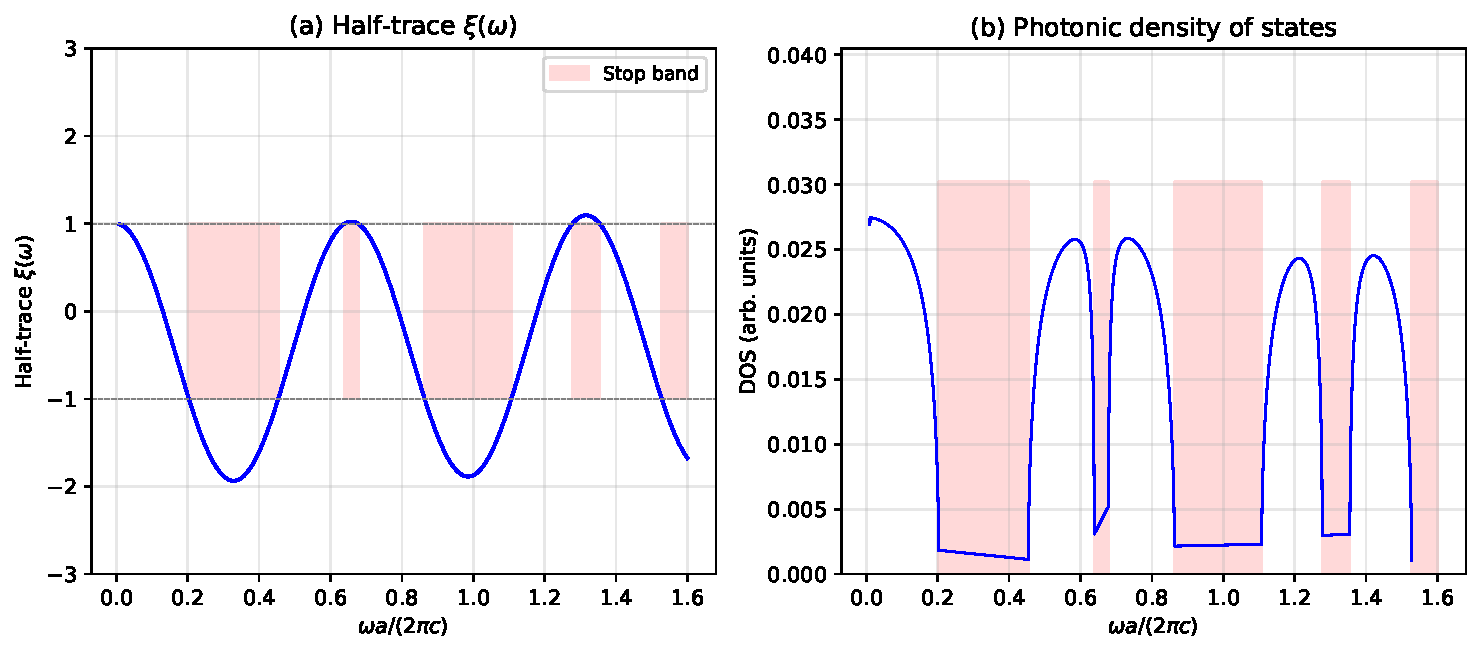
\includegraphics[width=0.85\linewidth]{figures/fig_f01_photonic_dos.pdf}
 \caption{Photonic density of states for a one-dimensional periodic
 dielectric. (a)~The transfer-matrix half-trace $\xi(\omega)$ divides
 pass bands ($|\xi|<1$) from stop bands ($|\xi|>1$). (b)~The density
 of states vanishes in stop bands and develops van-Hove enhancements
 near band edges, illustrating how Maxwell eigenvalue spectra differ
 qualitatively from free-space mode counting.}
 \label{fig:photonic-dos}
\end{figure}

When $\epsr$ becomes complex, the PDOS must be generalized to account for
the finite linewidth of the modes. The local density of states (LDOS)
at position $\rr_0$ is related to the imaginary part of the Green tensor:
\begin{equation}
 \rho(\rr_0, \omega) = \frac{2\omega}{\pi c^2}\,
 \Im\!\bigl[\tr \mathbf{G}(\rr_0, \rr_0; \omega)\bigr],
 \label{eq:ldos-green}
\end{equation}
where $\mathbf{G}$ is the dyadic Green tensor of the Maxwell system.
Chapter~\ref{ch:qnm} shows how the Green tensor can be expanded in terms
of quasinormal modes, providing a modal decomposition of the LDOS even
in open, non-Hermitian systems.


%% ================================================================
\section{What this book will build}
\label{sec:overview}

The rest of this monograph develops the consequences of the spectral
structure introduced here. Part~I continues by establishing the energy
inner products and reciprocity relations that underpin Hermitian photonics
(Chapter~\ref{ch:energy-inner}), deriving the Bloch band structure of
periodic media (Chapter~\ref{ch:periodicity}), and introducing the
scattering framework for open systems (Chapter~\ref{ch:boundaries}).

Part~II identifies the physical origins of non-Hermiticity:
material loss and gain (Chapter~\ref{ch:loss-gain-dispersion}),
radiation-induced complex eigenfrequencies in quasinormal modes
(Chapter~\ref{ch:qnm}), and the projection from the full Maxwell
operator to finite-dimensional coupled-mode models
(Chapter~\ref{ch:maxwell-coupled-modes}).

Part~III examines the most striking consequences of non-Hermitian operators:
exceptional points where eigenvectors coalesce
(Chapter~\ref{ch:exceptional-points}), $\PT$-symmetric optics
(Chapter~\ref{ch:pt-symmetric}), and the interplay of scattering poles
and zeros that connects lasers to coherent perfect absorbers
(Chapter~\ref{ch:poles-zeros}).

Part~IV builds the topological theory~\cite{icon2019rev,haldane2008possible}, starting from Berry curvature
derived directly from Maxwell fields (Chapter~\ref{ch:berry-maxwell}),
extending to complex bands and non-Hermitian gaps
(Chapter~\ref{ch:complex-bands}), developing photonic point-gap topology
(Chapter~\ref{ch:point-gap}), the skin effect and non-Bloch band theory
(Chapter~\ref{ch:skin-effect}), the reconstruction of bulk-boundary
correspondence (Chapter~\ref{ch:bbc-rebuilt}), and the topology of
bound states in the continuum (Chapter~\ref{ch:bic-topology}).

Part~V addresses computation (Chapter~\ref{ch:numerics}), devices and
physical limits (Chapter~\ref{ch:devices}), and open problems
(Chapter~\ref{ch:open-problems}).

Throughout, we shall insist on a single discipline: every non-Hermitian
structure must be traceable to a property of the Maxwell operator, not
merely asserted by analogy with a tight-binding Hamiltonian. This
Maxwell-first perspective is what gives the monograph its coherence and,
we hope, its lasting value.
